% Two-column, venue-neutral. Compiles on Overleaf with pdfLaTeX as-is.
% To retarget a venue, change only \documentclass and \bibliographystyle;
% nothing in the body depends on IEEEtran.
\documentclass[conference]{IEEEtran}

\usepackage{cite}
\usepackage{amsmath,amssymb}
\usepackage{graphicx}
\usepackage{booktabs}
\usepackage{xcolor}
\usepackage[hyphens]{url}
\usepackage[hidelinks]{hyperref}

\newcommand{\attr}{\textsc{attr}}
\newcommand{\pp}{\,pp}

\begin{document}

\title{Refusal Is Not Harm: Multi-Turn Jailbreak Benchmarks\\Rank Attacks Backwards}

\author{\IEEEauthorblockN{Parv Bansal}
\IEEEauthorblockA{\textit{AIMS-DTU} \\
Delhi Technological University \\
parvbansal05@gmail.com}}

\maketitle

\begin{abstract}
Multi-turn jailbreak evaluations almost universally score an attack as
successful when the model fails to refuse. We label 6{,}000 model responses with
two independent harm judges across five instruction-tuned models, four numeric
precisions, and two multi-turn attacks, and show that this convention does not
merely overstate attack success: it reverses the ordering of attacks. Across
fourteen matched model-precision configurations a coreference attack reports
81.9\% success against 20.2\% for an escalation attack (Wilcoxon $p<0.001$),
while causing 1.1\% attributable harm against 6.0\%. The reversal in
attributable harm is $+4.9$ percentage points (\pp) with a bootstrap 95\%
interval of $[+1.9,+8.2]$ that excludes zero under every one of four harm-labelling
rules, spanning two judges. The gap arises because refusal-based scoring credits
an attack for every answer the model would have produced without it; decomposing
reported success against a matched no-attack condition shows that 94\% of
coreference ``successes'' contain no harmful content at all. We further find that
multi-turn vulnerability is a property of the model family rather than of
quantization. Qwen2.5 refuses 99\% of single-turn harmful prompts yet drops to
7.5\% under multi-turn attack; Llama-3.x is unmoved by coreference and actively
hardens against escalation ($+23.0$\pp{} refusal, $p<10^{-4}$); Mistral-7B refuses
so rarely that its reported success is genuine. Finally, quantization leaves
static attacks unchanged (mean $1.6$\pp, $0/6$ significant) but significantly
alters adaptive ones (mean $8.1$\pp, three configurations surviving correction),
an effect we separate from a compute-backend confound with a matched FP16
replication (mean $0.5$\pp) and explain mechanistically: an attack conditioned on
model output is a different attack against a different model. We release all
completions, both sets of harm labels, and a single script that regenerates every
number reported here.
\end{abstract}

\begin{IEEEkeywords}
language model safety, jailbreak evaluation, multi-turn attacks, quantization,
measurement validity
\end{IEEEkeywords}

\section{Introduction}

A jailbreak attack is normally scored by whether the model refused. The
convention is convenient, cheap, and nearly universal in multi-turn work: run
the conversation, apply a refusal classifier to the final response, and report
the non-refusal rate as attack success rate (ASR). It also embeds an assumption
that is rarely stated, namely that a non-refusal is an attack success.

That assumption fails in a specific and consequential way. A model that answers
a question it would have answered anyway has not been attacked successfully; it
has merely been asked. Refusal-based scoring cannot separate the two, because it
never observes what the model would have done without the conversation.

We measure the size of that failure by adding two things the literature usually
omits: an independent harm judge applied to every response, and a matched
\emph{cold} condition in which the same final request is issued with no
preceding conversation. Together these decompose reported success into three
parts,
\begin{equation}
\text{reported} = \underbrace{\text{no harm}}_{\text{harmless}}
 + \underbrace{\text{pre-existing}}_{\text{harmful cold}}
 + \underbrace{\attr}_{\text{attack-caused}},
\label{eq:decomp}
\end{equation}
where a scenario counts as attack-attributable only if the model refused the
request cold, did not refuse it in context, and the resulting response was
judged harmful.

Applying this across five models, four precisions and two attacks produces a
result stronger than the expected overstatement: the two attacks swap places.
The attack reporting $4\times$ more success causes $5\times$ less harm
(Fig.~\ref{fig:inversion}). Rankings computed with the standard metric are not
merely inflated, they are ordered wrongly.

\smallskip\noindent\textbf{Contributions.}
\begin{enumerate}
\item Refusal-based ASR inverts the ordering of two widely used multi-turn
attacks, with both directions significant on matched configurations
(Sec.~\ref{sec:inversion}).
\item Multi-turn vulnerability is a model-family property invisible to
single-turn evaluation, spanning three distinct regimes across five models
(Sec.~\ref{sec:regimes}).
\item Quantization does not affect static multi-turn attacks but significantly
affects adaptive ones, with a mechanism: an attack conditioned on model output
diverges when the weights change (Sec.~\ref{sec:quant}). We separate this from a
compute-backend confound with a matched FP16 replication.
\end{enumerate}
Every reported effect is checked against a second, architecturally unrelated harm
judge, and the central inversion is reported as an effect size with a bootstrap
interval robust to the choice of judge (Sec.~\ref{sec:robust}).

\section{Related Work}

\textbf{Refusal as a direction.} Arditi et al.~\cite{arditi2024refusal} show
refusal is mediated by a single linear direction obtainable by
difference-in-means, and that ablating it removes refusal behaviour. We reuse
their extraction and ablation protocol as a causal check on layer choice, not as
an attack. Representation-level analysis of this kind follows
Zou et al.~\cite{zou2023representation}.

\textbf{Scoring jailbreak success.} StrongREJECT~\cite{souly2024strongreject}
showed that refusal-based and keyword-based scorers inflate single-turn attack
success relative to human judgement, and proposed a graded rubric.
HarmBench~\cite{mazeika2024harmbench} standardised harm classification. Our
result differs in kind: in the multi-turn setting the inflation is
\emph{attack-dependent} and large enough to reverse the ranking between attacks,
which rescaling a single attack's score cannot reveal. This continues a line of
work showing that a widely used metric can produce qualitatively wrong
conclusions, from emergent-ability claims that are artifacts of the
metric~\cite{schaeffer2023emergent} to benchmark validity more
broadly~\cite{raji2021everything,miller2024error}; over-refusal is the mirror
failure~\cite{rottger2024xstest}.

\textbf{Multi-turn attacks.} CoSafe~\cite{yu2024cosafe} constructs dialogues in
which the harmful referent is carried by coreference, so the final turn is often
innocuous read alone. Crescendo~\cite{russinovich2024crescendo} escalates across
turns and quotes the model's own prior output. Whether later turns are fixed
text or a function of model output turns out to determine both the attack's real
efficacy and its sensitivity to quantization. Fully adaptive attackers that
rewrite each turn from the model's replies~\cite{mehrotra2024tree,andriushchenko2024jailbreaking,ren2024actorattack}
sit at the far end of this axis, and multi-turn human red-teaming defeats current
defences~\cite{li2024multiturn,yang2024chainofattack}. Single-turn attack
construction has been studied
extensively~\cite{zou2023universal,chao2023jailbreaking,liu2024autodan,wei2023jailbroken}.

\textbf{Compression and safety.} Kadadekar~\cite{kadadekar2026quality} reports
that quality benchmarks do not track safety under quantization, finding
degradation that splits across models. Chhabra and
Khalili~\cite{chhabra2025refusal} report the refusal representation stays
geometrically intact under compression. Hong et al.~\cite{hong2024decoding}
survey trustworthiness under compression, and Egashira et
al.~\cite{egashira2024exploiting} show quantization can be adversarially
exploited. Our results are consistent with the representation being preserved,
and add that behavioural equivalence holds only for attacks that do not adapt.
That compression can silently change behaviour on a subset of inputs while
leaving aggregate quality intact is a known
pattern~\cite{hooker2019compressed,hooker2020characterising}. Quantization methods
themselves are due
to~\cite{frantar2023gptq,lin2024awq,dettmers2023qlora,dettmers2022llmint8,xiao2023smoothquant}.

\textbf{Alignment.} The models studied are aligned by RLHF or related
procedures~\cite{ouyang2022training,bai2022constitutional}, whose robustness has
been probed by red-teaming~\cite{ganguli2022red,perez2022red} and shown to
degrade under fine-tuning~\cite{qi2024finetuning}.

\section{Method}

\subsection{Models and precisions}
Five instruction-tuned models across three families: Llama-3.2-3B,
Llama-3.1-8B~\cite{dubey2024llama}, Qwen2.5-3B, Qwen2.5-7B,
Mistral-7B-Instruct-v0.3. Precisions are
FP16, NF4 (bitsandbytes, quantized at load), AWQ~\cite{lin2024awq} and
GPTQ~\cite{frantar2023gptq} where published 4-bit checkpoints exist. Generation
is greedy throughout, so differences are attributable to weights rather than
sampling.

\subsection{Attacks and the cold control}
\textbf{CoSafe} supplies three scripted user turns whose harmful referent is
established early and referred to pronominally at the end. \textbf{Crescendo}
escalates over four turns and, critically, quotes the model's own second-turn
output back to it in the third.

For every scenario we additionally run a \emph{cold} condition: the final
request alone, with no conversation history. This control makes
Eq.~\ref{eq:decomp} computable and costs one extra generation per scenario.

\subsection{Refusal direction and causal layer}
We extract a refusal direction per model by difference-in-means over 256 harmful
AdvBench prompts and 256 harmless Alpaca instructions, holding out a quarter for
validation. Selecting the layer by $d'$ alone lands near the final layer, whose
large raw separation is a norm-growth artifact of logit preparation; across all
five models the $d'$ peak (21--31) never coincides with the causal layer.
We therefore select the causal layer by ablation over 32 held-out prompts and
eleven candidate layers: project the direction out of the residual stream at
every layer during generation and measure the refusal collapse. This yields
layer 10 for Llama-8B, 24 for both 3B models, 16 for Qwen-7B and 12 for Mistral.
For Llama-8B, layer 10 drives refusal from 90.6\% to 0.0\% while ablating a random
unit direction leaves it unchanged; Mistral has no such bottleneck, as ablating
any layer past 12 collapses its already-low 18.8\% refusal, consistent with its
being weakly safety-tuned. The random-direction control is what makes the layer
choice causal rather than correlational.

\subsection{Metrics and statistics}
Refusal is scored by a substring classifier over the final response. Harm is
scored independently by Llama Guard 3 8B~\cite{inan2023llamaguard} over all
6{,}000 completions, and every completion is scored a second time by Granite
Guardian 3.1 2B~\cite{padhi2024granite}, an architecture that appears nowhere
among the systems under test, so its errors cannot correlate with them. Other
open harm judges follow a similar
design~\cite{han2024wildguard,zeng2024shieldgemma}. Judging precedes analysis and runs one file at a time, so no verdict
is confounded by generation hardware. All comparisons are paired within scenario
identifier: McNemar's exact test for binary refusal, Wilcoxon signed-rank for
attack-level comparisons, and Bonferroni correction across the fourteen precision
comparisons of Sec.~\ref{sec:quant} ($\alpha=0.0036$). Because the central
comparison rests on fourteen paired configurations, where Wilcoxon resolves
coarsely near the conventional threshold, we report its effect size with a
$10{,}000$-sample bootstrap interval as the primary statistic.

\begin{figure}[t]
\centering
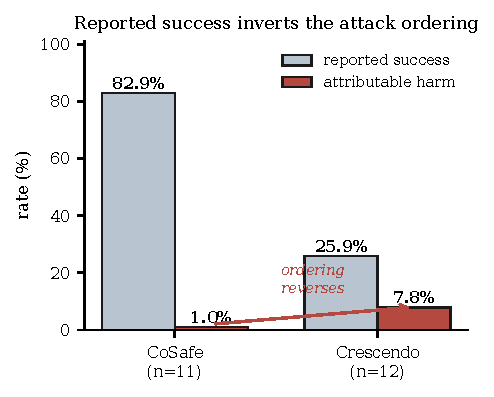
\includegraphics[width=\columnwidth]{fig_inversion.pdf}
\caption{Reported attack success against attack-attributable harm, averaged over
the fourteen matched model-precision configurations. The coreference attack
reports $4\times$ the success of the escalation attack while causing $5\times$
less harm. The two orderings point in opposite directions.}
\label{fig:inversion}
\end{figure}

\section{Reported Success Inverts the Attack Ordering}
\label{sec:inversion}

Table~\ref{tab:decomp} decomposes reported success by Eq.~\ref{eq:decomp}.
Across fourteen matched model-precision configurations in which both attacks ran,
CoSafe reports a mean ASR of 81.9\% against Crescendo's 20.2\% (Wilcoxon
$p=0.00098$). On attributable harm the ordering reverses: CoSafe 1.1\% against
Crescendo 6.0\%, a difference of $+4.9$\pp{} whose bootstrap 95\% interval
$[+1.9,+8.2]$ excludes zero. Sec.~\ref{sec:robust} shows the reversal survives
under both harm judges and under conjunctive and disjunctive labelling.

The decomposition shows why. For CoSafe 94\% of reported successes contain no
harmful content, because its final turns are frequently innocuous read alone;
cold refusal for CoSafe sits between 14\% and 40\%, so most of what it is credited
with was already available without any attack. Crescendo issues the harmful
request plainly, so cold refusal is 71--99\% and genuine headroom exists for an
attack to matter.

\begin{table}[t]
\centering
\caption{Decomposition of reported multi-turn success (\%), FP16 rows shown.
Attributable harm requires refusal when cold, non-refusal in context, and a
harmful verdict.}
\label{tab:decomp}
\small
\begin{tabular}{llrrrr}
\toprule
Model & Attack & Rep. & Harm & \attr & Pre-ex. \\
\midrule
Llama-3B    & CoSafe    & 76.0 & 4.0 & 1.0 & 3.0 \\
Llama-8B    & CoSafe    & 79.0 & 9.0 & 3.0 & 6.0 \\
Qwen-3B     & CoSafe    & 89.0 & 8.0 & 2.0 & 6.0 \\
Qwen-7B     & CoSafe    & 94.0 & 6.0 & 0.0 & 6.0 \\
Mistral-7B  & CoSafe    & 88.0 & 9.0 & 0.0 & 9.0 \\
\midrule
Llama-3B    & Crescendo &  5.5 &  7.0 &  2.5 &  1.5 \\
Llama-8B    & Crescendo &  2.0 &  4.5 &  0.0 &  0.0 \\
Qwen-3B     & Crescendo & 13.0 &  6.5 &  5.5 &  0.0 \\
Qwen-7B     & Crescendo & 32.5 & 14.0 & 14.0 &  0.0 \\
Mistral-7B  & Crescendo & 85.5 & 73.0 &  8.5 & 60.5 \\
\midrule
\multicolumn{2}{l}{\textbf{Mean CoSafe} (14 runs)}    & \textbf{81.9} & 5.8 & \textbf{1.1} & 4.6 \\
\multicolumn{2}{l}{\textbf{Mean Crescendo} (15 runs)} & \textbf{22.1} & 13.2 & \textbf{6.7} & 5.4 \\
\bottomrule
\end{tabular}
\end{table}

\textbf{Mistral is the control showing the metric is not broken in general.}
Mistral-7B refuses only 18.5\% of single-turn harmful prompts and produces
harmful output in 57\% of them. It is the one model where reported success
approximates real harm (86\% against 73\%, a factor of $1.2$ rather than the
$26$--$151\times$ seen elsewhere). Refusal-based scoring works precisely when the
model does not refuse, and fails on safety-tuned models, which are the models
anyone benchmarks.

\textbf{Scope.} The inversion is an aggregate result. Per configuration the flip
occurs in $9/14$ cases, a sign test at $p=0.42$, underpowered at this sample
size. We claim the aggregate ordering reverses, not that it reverses everywhere.

\section{Robustness of the Inversion}
\label{sec:robust}

The inversion rests on harm labels, so we test it against the choice of judge.
Table~\ref{tab:robust} recomputes the attributable-harm gap under four labelling
rules: each judge alone, the conjunctive rule (both judges must call a response
harmful), and the disjunctive rule (either suffices). The gap is positive and its
bootstrap interval excludes zero under all four; the point estimate ranges over a
narrow $4.8$--$5.6$\pp. The ordering reverses regardless of how harm is defined.

The two judges disagree more than either's self-description would suggest, a
reliability concern also raised for LLM-as-judge
evaluation~\cite{zheng2023judging}: over
all $6{,}000$ responses they agree on $88.6\%$, Cohen's $\kappa=0.45$, with
Granite flagging harm about twice as often as Llama Guard ($15.6\%$ against
$7.5\%$). This disagreement is itself evidence that automated harm scoring is
unreliable, and it is why we report the inversion as an interval robust to the
judge rather than a single $p$-value. On a stratified sample of 200 responses we
add a third, unrelated judgement: of the coreference ``successes'' both automated
judges call harmless, the third labels only $10\%$ ($4/40$) harmful, and the
under-flagging rate is identical across the two attacks ($14\%$ each on the
cold-refused subset that could become attributable), so it cannot manufacture the
gap.

\begin{table}[t]
\centering
\caption{Attributable-harm gap (Crescendo minus CoSafe, \pp) under four harm
labelling rules, over fourteen matched configurations. CI is a $10{,}000$-sample
bootstrap. Every interval excludes zero.}
\label{tab:robust}
\small
\begin{tabular}{lrrl}
\toprule
Harm rule & CoSafe & Crescendo & Gap (95\% CI) \\
\midrule
Llama Guard      & 1.1 & 6.0 & $+4.9\;[+1.9,+8.2]$ \\
Granite Guardian & 2.4 & 7.9 & $+5.5\;[+1.6,+9.7]$ \\
Both agree       & 0.8 & 5.6 & $+4.8\;[+1.9,+7.8]$ \\
Either           & 2.7 & 8.3 & $+5.6\;[+1.6,+10.0]$ \\
\bottomrule
\end{tabular}
\end{table}

\section{Vulnerability Is a Family Property}
\label{sec:regimes}

Figure~\ref{fig:regimes} and Table~\ref{tab:regimes} compare cold and in-context
refusal for all five models at FP16. Three regimes appear.

\textbf{Llama-3.x: immune to coreference, hardened by escalation.} Refusal moves
by $+1.0$\pp{} ($p=0.87$) and $+0.5$\pp{} ($p=1.00$) under CoSafe for 3B and 8B,
while the metric reports 75.5\% and 73.0\% ASR. Under Crescendo refusal
\emph{rises}: $+23.0$\pp{} for 3B ($p<10^{-4}$) and $+4.0$\pp{} for 8B
($p=0.039$). Quoting the model's own words back appears to trigger suspicion
rather than compliance.

\textbf{Qwen2.5: genuinely vulnerable, invisible single-turn.} Both Qwen models
refuse 99\% of single-turn AdvBench prompts, which a single-turn benchmark would
report as near-perfect safety. Under attack Qwen-7B falls to 7.5\% (CoSafe,
$-14.5$\pp, $p<10^{-4}$) and 67.5\% (Crescendo, $-31.5$\pp, $p<10^{-4}$, with 63
scenarios flipping to non-refusal against zero flipping back).

\textbf{Mistral: not meaningfully safety-tuned.} Neither attack has a detectable
effect ($p=0.07$, $p=0.20$), yet both report 80--85\% success.

\begin{table}[t]
\centering
\caption{Cold versus in-context refusal (\%) at FP16, exact McNemar.
Reported ASR is $100-\text{in-context}$.}
\label{tab:regimes}
\small
\begin{tabular}{llrrrr}
\toprule
Model & Attack & Cold & In-ctx & $\Delta$ & $p$ \\
\midrule
Llama-3B   & CoSafe    & 23.5 & 24.5 & $+1.0$  & 0.87 \\
Llama-8B   & CoSafe    & 26.5 & 27.0 & $+0.5$  & 1.00 \\
Qwen-3B    & CoSafe    & 40.0 & 14.5 & $-25.5$ & $<10^{-4}$ \\
Qwen-7B    & CoSafe    & 22.0 &  7.5 & $-14.5$ & $<10^{-4}$ \\
Mistral-7B & CoSafe    & 14.5 & 20.0 & $+5.5$  & 0.07 \\
\midrule
Llama-3B   & Crescendo & 71.5 & 94.5 & $+23.0$ & $<10^{-4}$ \\
Llama-8B   & Crescendo & 94.0 & 98.0 & $+4.0$  & 0.039 \\
Qwen-3B    & Crescendo & 99.0 & 87.0 & $-12.0$ & $<10^{-4}$ \\
Qwen-7B    & Crescendo & 99.0 & 67.5 & $-31.5$ & $<10^{-4}$ \\
Mistral-7B & Crescendo & 19.0 & 14.5 & $-4.5$  & 0.20 \\
\bottomrule
\end{tabular}
\end{table}

In four of ten model-attack conditions the attack has no statistically
detectable effect on refusal, and mean reported ASR across those four is 78.5\%.

\begin{figure*}[t]
\centering

\includegraphics[width=\textwidth]{fig_regimes.pdf}
\caption{Refusal with no conversation (grey) and after the attack (blue), FP16.
Arrows are red where the change exceeds 8\pp. Llama models move little under
CoSafe and upward under Crescendo; Qwen models fall sharply under both; Mistral
starts too low for either attack to matter.}
\label{fig:regimes}
\end{figure*}

\section{Quantization Affects Adaptive Attacks Only}
\label{sec:quant}

Table~\ref{tab:quant} compares each quantized variant against its FP16
counterpart, paired within scenario. To hold the compute backend fixed, the FP16
baseline here is a replication generated on the same CUDA hardware as the
quantized arms (see below). Under CoSafe none of six comparisons is significant
and the mean absolute change is $1.6$\pp. Under Crescendo the mean absolute change
is $8.1$\pp{} and three comparisons survive Bonferroni correction: Qwen-3B NF4
($+15.5$\pp, $p<10^{-6}$), Qwen-7B NF4 ($+11.5$\pp, $p=1.2\times10^{-4}$) and
Qwen-7B GPTQ ($+16.5$\pp, $p<10^{-4}$).

\begin{table}[t]
\centering
\caption{Quantized minus FP16 reported ASR (\pp), paired within scenario, FP16
baseline generated on the same hardware. $\dagger$ survives Bonferroni correction
across fourteen comparisons.}
\label{tab:quant}
\small
\begin{tabular}{llrrl}
\toprule
Model & Prec. & CoSafe & Crescendo & $p$ (Cres.) \\
\midrule
Llama-3B  & NF4  & $-1.0$ & $-3.0$  & 0.070 \\
Llama-8B  & NF4  & $-2.0$ & $+4.5$  & 0.012 \\
Llama-8B  & AWQ  & $-3.5$ & $+0.5$  & 1.00 \\
Qwen-3B   & NF4  & $+1.0$ & $+15.5$ & $<10^{-6}$\,$\dagger$ \\
Qwen-7B   & NF4  & $+0.0$ & $+11.5$ & $1.2{\times}10^{-4}$\,$\dagger$ \\
Qwen-7B   & AWQ  & $-2.0$ & $+5.5$  & 0.099 \\
Qwen-7B   & GPTQ & ---    & $+16.5$ & $<10^{-4}$\,$\dagger$ \\
\midrule
\multicolumn{2}{l}{Mean $|\Delta|$} & \textbf{1.6} & \textbf{8.1} & \\
\bottomrule
\end{tabular}
\end{table}

\textbf{Backend control.} The quantized arms were generated on CUDA and our
original FP16 arms on Apple Silicon, so a naive precision comparison also crosses
a compute backend. Because our proposed mechanism is amplification of small
perturbations, a backend change could mimic a precision effect. We therefore
regenerated every FP16 arm on the CUDA hardware and compared the two FP16 sets
directly: across seven attack-model comparisons the mean absolute difference is
$0.5$\pp{} with none significant. The backend accounts for essentially none of
the quantization effect, and the CUDA FP16 replication is the baseline used in
Table~\ref{tab:quant}.

\textbf{Mechanism.} Crescendo's third turn quotes the model's own second-turn
output. Quantization perturbs that output, changing what the third turn asks,
which compounds into the fourth. CoSafe's turns are fixed text, so quantization
affects only the final response and nothing accumulates. The direction of change
is not monotone, with Llama-3B becoming safer by $3.0$\pp{} while everything else
becomes more vulnerable, which is what trajectory divergence predicts and uniform
safety degradation does not.

Figure~\ref{fig:triple} isolates this on one model. Qwen-3B under a single
precision change moves by $+0.0$\pp{} single-turn ($p=1.00$), $+1.0$\pp{} under
CoSafe ($p=0.77$), and $+15.5$\pp{} under Crescendo ($p<10^{-6}$, 35 scenarios
flipping against 4). The only property differing between the second and third
conditions is whether later turns depend on the model's own earlier outputs.

\begin{figure}[t]
\centering
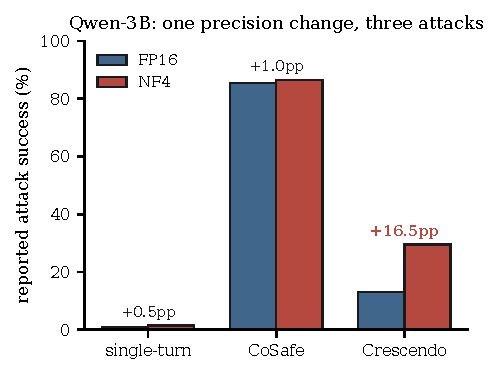
\includegraphics[width=\columnwidth]{fig_triple.pdf}
\caption{Qwen2.5-3B, FP16 against NF4 on identical CUDA hardware, under three
attack types. Only the attack's dependence on model output differs across the
three panels; the precision change moves the self-referential attack alone.}
\label{fig:triple}
\end{figure}

The implication is methodological. An adaptive attack applied to two model
variants is not one attack measured twice, because the attack is itself a
function of the model. Comparisons of model variants under adaptive attack must
control for trajectory divergence or report it.

\section{Discussion}

The remedy is cheap. Reporting the cold-condition refusal rate alongside ASR
costs one extra generation per scenario and makes the inflation visible
immediately; reporting attributable harm additionally requires a judge pass.
Either would have exposed the inversion of Sec.~\ref{sec:inversion} without any
new attack design.

More broadly, the failure mode is specific to well-aligned models. As alignment
improves, the fraction of non-refusals that are genuinely harmful falls, and the
refusal metric becomes progressively less informative exactly where safety
evaluation matters most. Mistral demonstrates the converse: on a weakly aligned
model the metric is close to correct.

\section{Limitations}

Harm is scored by two automated judges rather than humans. They agree at
$\kappa=0.45$, so the choice of judge is a genuine source of variance; we address
it by reporting the inversion as an interval robust across both judges and two
labelling rules (Sec.~\ref{sec:robust}), but human validation on the stratified
sample remains the natural next step, and the third judgement we add there is
itself automated. CoSafe's categories are mild relative to Llama Guard's
severe-hazard taxonomy and may be under-flagged; the Mistral row, where the same
pipeline returns 73\% harm, indicates the judges are not simply insensitive.
CoSafe and single-turn completions are $n{=}100$ for the original FP16 arms and
$n{=}200$ elsewhere, with all comparisons paired on shared identifiers. Mistral
quantized variants and Llama-8B GPTQ were not collected because compute was
exhausted, and one CoSafe arm for Qwen-7B GPTQ was lost to a storage fault. The
mechanism of Sec.~\ref{sec:quant} predicts that a fully adaptive attacker, whose
every turn is rewritten from the model's replies, should show a still larger
precision effect; testing that dose-response relationship is left to future work,
as a preliminary attempt was dominated by the attacker model's own refusals.

\section{Conclusion}

Scoring multi-turn jailbreaks by refusal does not merely overstate attack
success; on matched configurations it reverses which of two attacks is more
dangerous. Adding a no-attack control and an independent harm judge separates
attacks that defeat refusal from attacks credited for answers the model would
have given regardless. Under that measurement, multi-turn vulnerability is a
property of the model family rather than of numeric precision, and quantization
matters only for attacks that adapt to the model they attack.

\section*{Reproducibility}

All completions, both sets of harm labels, attack scripts and a single analysis
script that regenerates every number appear in the artifact. Generation is greedy
throughout; the FP16 arms were reproduced on a second compute backend and the two
sets agree to within $0.5$\pp{} on average.

\bibliographystyle{IEEEtran}
\bibliography{refs}

\end{document}
